% move all configuration stuff into one file so we can focus on the content
\documentclass[aspectratio=169,hyperref={pdfpagelabels=false,colorlinks=true,linkcolor=white,urlcolor=lightblue},xcolor={table},t]{beamer}

%%%%%%%%%%%%%%%%%%%%%%%%%%%%%%%%%%%%%%%%%%%%%%%%%%%%%%%%%%%%%%%%%%%%%%%%%%%%%%%%%%
%%%%%%%%%%%%%%%%%%%%%%%%%%%%%%%%%%%%%%%%%%%%%%%%%%%%%%%%%%%%%%%%%%%%%%%%%%%%%%%%%%
% packages
\usepackage{pict2e}
\usepackage{epic}
\usepackage{amsmath,amsfonts,amssymb}
\usepackage{units}
\usepackage{fancybox}
\usepackage[absolute,overlay]{textpos} 
%\usepackage[table]{xcolor}
\usepackage{animate}
\usepackage{gensymb}
%\usepackage{graphicx}
%\usepackage{longtable}
\usepackage{multirow}
\usepackage{silence}
\usepackage{tikz}
\usepackage[backend=bibtex,style=ieee]{biblatex}
\AtEveryCitekey{\iffootnote{\tiny}{}}
%\addbibresource{include/references}



% fontsize
\let\Tiny=\tiny

%%%%%%%%%%%%%%%%%%%%%%%%%%%%%%%%%%%%%%%%%%%%%%%%%%%%%%%%%%%%%%%%%%%%%%%%%%%%%%%%%%
%%%%%%%%%%%%%%%%%%%%%%%%%%%%%%%%%%%%%%%%%%%%%%%%%%%%%%%%%%%%%%%%%%%%%%%%%%%%%%%%%%
% warnings
\pdfsuppresswarningpagegroup=1
\WarningFilter{biblatex}{Patching footnotes failed}
\WarningFilter{latexfont}{Font shape}
\WarningFilter{latexfont}{Some font shapes}
\WarningFilter{gensymb}{Not defining}


%%%%%%%%%%%%%%%%%%%%%%%%%%%%%%%%%%%%%%%%%%%%%%%%%%%%%%%%%%%%%%%%%%%%%%%%%%%%%%%%%%
%%%%%%%%%%%%%%%%%%%%%%%%%%%%%%%%%%%%%%%%%%%%%%%%%%%%%%%%%%%%%%%%%%%%%%%%%%%%%%%%%%
% colors
\definecolor{gtgold}{rgb}{.914, .664, 0} %0e7eed {rgb}{0.88,0.66,1,0.06} [234, 170, 0]/256 %96caff
\definecolor{darkgray}{rgb}{.15, .15, .15}
\definecolor{lightblue}{HTML}{0e7eed}
\definecolor{highlight}{rgb}{0, 0, 1} %_less!40

%%%%%%%%%%%%%%%%%%%%%%%%%%%%%%%%%%%%%%%%%%%%%%%%%%%%%%%%%%%%%%%%%%%%%%%%%%%%%%%%%%
%%%%%%%%%%%%%%%%%%%%%%%%%%%%%%%%%%%%%%%%%%%%%%%%%%%%%%%%%%%%%%%%%%%%%%%%%%%%%%%%%%
% relative paths
\graphicspath{{../graph/}}


%%%%%%%%%%%%%%%%%%%%%%%%%%%%%%%%%%%%%%%%%%%%%%%%%%%%%%%%%%%%%%%%%%%%%%%%%%%%%%%%%%
%%%%%%%%%%%%%%%%%%%%%%%%%%%%%%%%%%%%%%%%%%%%%%%%%%%%%%%%%%%%%%%%%%%%%%%%%%%%%%%%%%
% units
\setlength{\unitlength}{1mm}

%%%%%%%%%%%%%%%%%%%%%%%%%%%%%%%%%%%%%%%%%%%%%%%%%%%%%%%%%%%%%%%%%%%%%%%%%%%%%%%%%%
%%%%%%%%%%%%%%%%%%%%%%%%%%%%%%%%%%%%%%%%%%%%%%%%%%%%%%%%%%%%%%%%%%%%%%%%%%%%%%%%%%
% math
\DeclareMathOperator*{\argmax}{argmax}
\DeclareMathOperator*{\argmin}{argmin}
\DeclareMathOperator*{\atan}{atan}
\DeclareMathOperator*{\arcsinh}{arcsinh}
\DeclareMathOperator*{\sign}{sign}
\DeclareMathOperator*{\tcdf}{tcdf}
\DeclareMathOperator*{\si}{sinc}
\DeclareMathOperator*{\princarg}{princarg}
\DeclareMathOperator*{\arccosh}{arccosh}
\DeclareMathOperator*{\hwr}{HWR}
\DeclareMathOperator*{\flip}{flip}
\DeclareMathOperator*{\sinc}{sinc}
\DeclareMathOperator*{\floor}{floor}
\newcommand{\e}{{e}}
\newcommand{\jom}{\mathrm{j}\omega}
\newcommand{\jOm}{\mathrm{j}\Omega}
\newcommand   {\mat}[1]    		{\boldsymbol{\uppercase{#1}}}		%bold
\renewcommand {\vec}[1]    		{\boldsymbol{\lowercase{#1}}}		%bold

%%%%%%%%%%%%%%%%%%%%%%%%%%%%%%%%%%%%%%%%%%%%%%%%%%%%%%%%%%%%%%%%%%%%%%%%%%%%%%%%%%
%%%%%%%%%%%%%%%%%%%%%%%%%%%%%%%%%%%%%%%%%%%%%%%%%%%%%%%%%%%%%%%%%%%%%%%%%%%%%%%%%%
% media9
\newcommand{\includeaudio}[1]{
\href{run:audio/#1.mp3}{
\includegraphics[width=5mm, height=5mm]{graph/SpeakerIcon}}}

\newcommand{\includeanimation}[4]{{\begin{center}
                        \animategraphics[autoplay,loop,scale=.7]{#4}{animation/#1-}{#2}{#3}        
                        \end{center}
                        \addreference{matlab source: \href{https://github.com/alexanderlerch/ACA-Plots/blob/master/matlab/animate#1.m}{matlab/animate#1.m}}}
                        \inserticon{video}}
                        
%%%%%%%%%%%%%%%%%%%%%%%%%%%%%%%%%%%%%%%%%%%%%%%%%%%%%%%%%%%%%%%%%%%%%%%%%%%%%%%%%%
%%%%%%%%%%%%%%%%%%%%%%%%%%%%%%%%%%%%%%%%%%%%%%%%%%%%%%%%%%%%%%%%%%%%%%%%%%%%%%%%%%
% other commands
\newcommand{\question}[1]{%\vspace{-4mm}
                          \setbeamercovered{invisible}
                          \begin{columns}[T]
                            \column{.9\textwidth}
                                \textbf{#1}
                            \column{.1\textwidth}
                                \vspace{-8mm}
                                \begin{flushright}
                                     
\includegraphics[width=.9\columnwidth]{graph/question_mark}
                                \end{flushright}
                                \vspace{6mm}
                          \end{columns}\pause\vspace{-12mm}}

\newcommand{\toremember}[1]{
                        \inserticon{lightbulb}
                        }

\newcommand{\matlabexercise}[1]{%\vspace{-4mm}
                          \setbeamercovered{invisible}
                          \begin{columns}[T]
                            \column{.8\textwidth}
                                \textbf{matlab exercise}: #1
                            \column{.2\textwidth}
                                \begin{flushright}
                                     \includegraphics[scale=.5]{graph/logo_matlab}
                                \end{flushright}
                                %\vspace{6mm}
                          \end{columns}}

\newcommand{\addreference}[1]{  
                  
                    \begin{textblock*}{\baselineskip }(.98\paperwidth,.5\textheight) %(1.15\textwidth,.4\textheight)
                         \begin{minipage}[b][.5\paperheight][b]{1cm}%
                            \vfill%
                             \rotatebox{90}{\tiny {#1}}
                        \end{minipage}
                   \end{textblock*}
                    }
                    
\newcommand{\figwithmatlab}[1]{
                    \begin{figure}
                        \centering
                        \includegraphics[scale=.7]{#1}
                        %\label{fig:#1}
                    \end{figure}
                    
                    \addreference{matlab source: \href{https://github.com/alexanderlerch/MUSI-6202/blob/main/matlab/plot#1.m}{plot#1.m}}}
\newcommand{\figwithref}[2]{
                    \begin{figure}
                        \centering
                        \includegraphics[scale=.7]{#1}
                        \label{fig:#1}
                    \end{figure}
                    
                    \addreference{#2}}  
                                    
\newcommand{\inserticon}[1]{
                    \begin{textblock*}{100mm}(14.5cm,7.5cm)
                        \includegraphics[height=.8cm,keepaspectratio]{graph/#1}
                    \end{textblock*}}            

%%%%%%%%%%%%%%%%%%%%%%%%%%%%%%%%%%%%%%%%%%%%%%%%%%%%%%%%%%%%%%%%%%%%%%%%%%%%%%%%%%
%%%%%%%%%%%%%%%%%%%%%%%%%%%%%%%%%%%%%%%%%%%%%%%%%%%%%%%%%%%%%%%%%%%%%%%%%%%%%%%%%%
% counters
\newcounter{i}
\newcounter{j}
\newcounter{iXOffset}
\newcounter{iYOffset}
\newcounter{iXBlockSize}
\newcounter{iYBlockSize}
\newcounter{iYBlockSizeDiv2}
\newcounter{iXBlockSizeDiv2}
\newcounter{iDistance}

\newcommand{\IEEELink}{https://ieeexplore.ieee.org/servlet/opac?bknumber=9965970}


\subtitle{Part 1: Organizational}

%%%%%%%%%%%%%%%%%%%%%%%%%%%%%%%%%%%%%%%%%%%%%%%%%%%%%%%%%%%%%%%%%%%%%%%%%%%%
\begin{document}
    % generate title page
	\title[]{Digital Signal Processing for Music}   
\author[alexander lerch]{alexander lerch} 
%\institute{~}
%\date[Alexander Lerch]{}
\titlegraphic{\vspace{-16mm}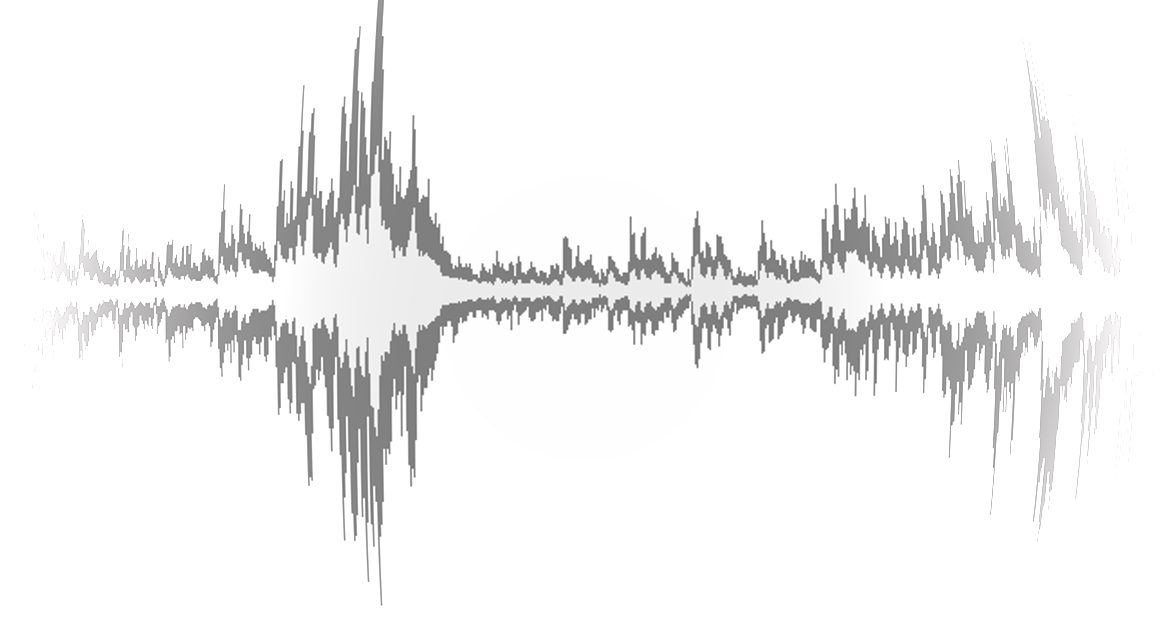
\includegraphics[width=\textwidth,height=3cm]{title}}


\begin{frame}
    \titlepage
    %\vspace{-5mm}
    \begin{flushright}
        \href{http://www.gtcmt.gatech.edu}{
\includegraphics[height=.8cm,keepaspectratio]{../shared/Logo_GTCMT_black}}
    \end{flushright}
\end{frame}


    \section[contact]{contact \& resources}
        \begin{frame}\frametitle{organizational}\framesubtitle{links \& contact}
            \begin{itemize}
                \item \textbf{contact info}
                    \begin{itemize}
                        \item   \textit{alexander lerch}
                            \begin{itemize}
                                \item   {email}: \url{mailto:alexander.lerch@gatech.edu}
                                \item   {www}: \url{www.audiocontentanalysis.org}
                                \item   {office}: Couch 205B
                                \item   {office hours}:  \textbf{by appointment}: \url{https://www.calendly.com/alexanderlerch}
                            \end{itemize}
                        %\item   \textit{teaching assistants}
                            %\begin{itemize}
                                %\item    Siddharth Gururani: \url{siddgururani@gatech.edu}
                                %\item    Ashis Pati: \url{ashis.pati@gatech.edu}
                            %\end{itemize}
                    \end{itemize}
                
                \smallskip
                \item<2-> \textbf{classes}
                    \begin{itemize}
                        \item   Mon, Wed  3:00--4:15pm in WV163
                        \item   additional \textit{tutorial group}: TBD
                    \end{itemize}
                
                \smallskip
                \item<3-> \textbf{class resources}
                    \begin{itemize}
                        \item	\textit{canvas}:
                            \begin{itemize}
                                \item   syllabus, grades, slides: \url{www.canvas.gatech.edu}
                            \end{itemize}
                    \end{itemize}
            \end{itemize}
        \end{frame}

    \section{course intro}
        \begin{frame}\frametitle{organizational}\framesubtitle{goals \& requirements}
            \begin{itemize}
                \item	\textbf{goals}
                        \begin{enumerate}
                            \item   ability to comprehend typical representations of digital systems such as block diagrams and difference equations,
                            \item   understanding of typical transforms in DSP such as the Fourier transform or the Z-transform,
                            \item    ability to use this understanding to design audio processing systems such as audio effects, and
                            \item	ability to implement such designs in a programming language such as Matlab.
                        \end{enumerate}

                \smallskip
                \item<2-> \textbf{requirements}	
                        \begin{itemize}
                            \item	math
                            \item	rudimentary programming skills, familiarity with Matlab
                        \end{itemize}
            \end{itemize}
        \end{frame}
        \begin{frame}\frametitle{organizational}\framesubtitle{outline}
            \vspace{-3mm}
            \begin{scriptsize}
                \begin{tabular}{l|p{.4\linewidth}|p{.1\linewidth}|p{.2\linewidth}||p{.1\linewidth}}
            \textbf{date} & \textbf{topics} & \textbf{exercise} & \textbf{assignment} & \textbf{notes}\\
            \hline\hline
            01/07 & introduction, signals, periodicity, random processes, pdf, moments, correlation & correlation &  &  \\
            01/14 & convolution, power spectral density & FIR filter& filter \& convolution & \\
            01/21 & Fourier series \& Fourier transform& DFT & Fourier analysis & MLK Hldy.\\
            01/28 &Fourier transform, sampling, quantization, SNR, number formats& quantization&& \\
            02/04 &oversampling, dither, noise-shaping, non-linear quant.&&dither, ns  & \\
            02/11 &z-transform, digital audio filters, FIR/IIR, FFT filtering& biquad& & midterm I\\
            02/18 &sample rate conversion, real-time systems &resampling&& \\
            02/25 &delay-based FX and reverb&vibrato& mod. fx&\\
            03/04 &dynamics processing& PPM & limiter & guthman\\
            03/11 &time-segment processing (OLA)&ola&& midterm II \\
            03/18 &&&&spring break \\
            03/25 &phase-vocoder&& phase voc&\\
            04/01 &source coding: LPC, ADPCM&&& \\
            04/08 &source coding: Huffman, AAC&&& \\
            04/15 &denoising&&& \\
            04/22 &competition results&&& \\
                \end{tabular}
            \end{scriptsize}
        \end{frame}

    \section{materials}
        \begin{frame}\frametitle{organizational}\framesubtitle{course materials}
        \begin{itemize}
            \item   \textbf{roughly based on}:  
                \begin{itemize}
                    \item   Z\"olzer, Udo (2008): \textit{Digital Audio Signal Processing}, Wiley 
                \end{itemize}
             \pause
             \bigskip
             \item   \textbf{additional  reading}:  
                \begin{itemize}
                    \item   Lyon, Richard (2011): \textit{Understanding Digital Signal Processing}, Prentice Hall 
                    \item   Z\"olzer, Udo (2011): \textit{DAFX: Digital Audio Effects}, Wiley
                \end{itemize}
            \pause
            \bigskip
            \item   \textbf{{additional} additional reading}:
                \begin{itemize}
                    \item   Pohlmann, Ken (2000): Principles of Digital Audio, 4th, McGraw-Hill
                    \item   Watkinson, John (2001): The Art of Digital Audio, Focal Press
                \end{itemize}

                %\only<1-2>{\vspace{5mm}
                %\begin{columns}[c]
                    %\column{.1\textwidth}
                    %\column{.3\textwidth}\includegraphics[scale=0.005]{graph/psychologyofhearing}
                    %\column{.3\textwidth}\includegraphics[scale=0.005]{graph/psychologyofmusic}
                    %\column{.3\textwidth}\includegraphics[scale=0.25]{graph/musicophilia}
                %\end{columns}}
            \pause
            \bigskip
            \item   \textbf{software}: 
                \begin{itemize}
                    \item   Matlab: \url{www.matlab.gatech.edu}
                    \item   github.com etc
                \end{itemize}
        \end{itemize}
       \end{frame}

    \section{assessment}
        \begin{frame}\frametitle{organizational}\framesubtitle{assessment}
            \begin{itemize}
                \item	\textbf{40\%: assignments} (equally weighted): projected deadlines see syllabus
                        \begin{enumerate}
                            \item	convolution and FIR filters
                            \item   Fourier analysis
                            \item   Dither \& Noise Shaping
                            \item   modulated audio effects
                            \item   compressor \& limiter
                            \item   (phase vocoder)
                        \end{enumerate}

                \smallskip
                \item   \textbf{10\%: mid-term exam I}
                \item   \textbf{10\%: mid-term exam II}

                \smallskip
                \item   \textbf{5\%: participation}

                \smallskip
                \item   \textbf{15\%: quizzes}
                    \begin{itemize}
                        \item   every week?! 
                    \end{itemize}
                
                \smallskip
                \item   \textbf{20\% codec competition}
            \end{itemize}
        \end{frame}

    \section{to do}
        \begin{frame}\frametitle{organizational}\framesubtitle{to do}
            \begin{enumerate}
                %\item   \textbf{find group partner}\\
                %mixed group (1st year + 2nd year) preferred
            
                \smallskip
                \item<2->   \textbf{install Matlab} (Octave/Freemat)
            
                \smallskip
                \item<3->   \textbf{brush up} your math and Matlab
            
            \end{enumerate}
        \end{frame}

\end{document}

